%% ****** Start of file apstemplate.tex ****** %
%%
%%
%%   This file is part of the APS files in the REVTeX 4 distribution.
%%   Version 4.1r of REVTeX, August 2010
%%
%%
%%   Copyright (c) 2001, 2009, 2010 The American Physical Society.
%%
%%   See the REVTeX 4 README file for restrictions and more information.
%%
%
% This is a template for producing manuscripts for use with REVTEX 4.0
% Copy this file to another name and then work on that file.
% That way, you always have this original template file to use.
%
% Group addresses by affiliation; use superscriptaddress for long
% author lists, or if there are many overlapping affiliations.
% For Phys. Rev. appearance, change preprint to twocolumn.
% Choose pra, prb, prc, prd, pre, prl, prstab, prstper, or rmp for journal
%  Add 'draft' option to mark overfull boxes with black boxes
%  Add 'showpacs' option to make PACS codes appear
%  Add 'showkeys' option to make keywords appear
\documentclass[aps,pre,reprint,superscriptaddress, twocolumn]{revtex4}
%\documentclass[aps,pre,preprint,superscriptaddress]{revtex4}
%\documentclass[aps,prl,reprint,groupedaddress]{revtex4}

% You should use BibTeX and apsrev.bst for references
% Choosing a journal automatically selects the correct APS
% BibTeX style file (bst file), so only uncomment the line
% below if necessary.
\bibliographystyle{apsrev4-1}

\usepackage{graphicx}
\usepackage{amsmath}
\usepackage{float}

\newcommand{\e}[1]{\times10^{#1}}
\newcommand{\gd}{\dot{\gamma}}
\newcommand{\com}[1]{{\bf {#1}}}

\begin{document}

% Use the \preprint command to place your local institutional report
% number in the upper righthand corner of the title page in preprint mode.
% Multiple \preprint commands are allowed.
% Use the 'preprintnumbers' class option to override journal defaults
% to display numbers if necessary
%\preprint{}

%Title of paper
\title{Rheology of Cubic Blue Phases}

% repeat the \author .. \affiliation  etc. as needed
% \email, \thanks, \homepage, \altaffiliation all apply to the current
% author. Explanatory text should go in the []'s, actual e-mail
% address or url should go in the {}'s for \email and \homepage.
% Please use the appropriate macro foreach each type of information

% \affiliation command applies to all authors since the last
% \affiliation command. The \affiliation command should follow the
% other information
% \affiliation can be followed by \email, \homepage, \thanks as well.

\author{O. Henrich}
\email[Corresponding author: ]{o.henrich@ucl.ac.uk}
\affiliation{EPCC, School of Physics and Astronomy, University of Edinburgh,\\JCMB Kings Buildings, Mayfield Road, Edinburgh EH9 3JZ, UK}
\affiliation{Centre for Computational Science, University College London,\\20 Gordon Street, London WC1H 0AJ, UK}

\author{K. Stratford}
\affiliation{EPCC, School of Physics and Astronomy, University of Edinburgh,\\JCMB Kings Buildings, Mayfield Road, Edinburgh EH9 3JZ, UK}

\author{P.V. Coveney}
\affiliation{Centre for Computational Science, University College London,\\20 Gordon Street, London WC1H 0AJ, UK}

\author{M.E. Cates}
\affiliation{SUPA, School of Physics and Astronomy, University of Edinburgh,\\JCMB Kings Buildings, Mayfield Road, Edinburgh EH9 3JZ, UK}

\author{D. Marenduzzo}
\affiliation{SUPA, School of Physics and Astronomy, University of Edinburgh,\\JCMB Kings Buildings, Mayfield Road, Edinburgh EH9 3JZ, UK}


%\homepage[]{Your web page}
%\thanks{}
%\altaffiliation{}

%Collaboration name if desired (requires use of superscriptaddress
%option in \documentclass). \noaffiliation is required (may also be
%used with the \author command).
%\collaboration can be followed by \email, \homepage, \thanks as well.
%\collaboration{}

%\noaffiliation

\date{\today}

\begin{abstract}
We study the behaviour of cubic blue phases under shear flow
via lattice Boltzmann simulations. We focus on the two experimentally observed
phases, Blue Phase I (BPI) and Blue Phase II (BPII). The disclination network of Blue Phase 
II continuously breaks and reforms under shear, leading to an oscillatory stress response in time.
\end{abstract}

% insert suggested PACS numbers in braces on next line
\pacs{47.11.Qr, 47.57.Lj, 47.57.Qk, 61.30.Dk, 61.30.Pq, 61.30.Jf, 83.80.Xz}
% insert suggested keywords - APS authors don't need to do this
\keywords{blue phase, cholesterics, chiral nematics, rheology}

%\maketitle must follow title, authors, abstract, \pacs, and \keywords
\maketitle

% body of paper here - Use proper section commands
% References should be done using the \cite, \ref, and \label commands
\section{Introduction}
% Put \label in argument of \section for cross-referencing
%\section{\label{}}

Cholesterics are liquid crystals in which the local nematic director field spontaneously 
twists in thermodynamic equilibrium~\cite{deGennes}. The preferred configuration close 
to the isotropic boundary features twist around two perpendicular axes, as opposed to 
just one axis in the regular cholesteric state, and the corresponding deformation is 
denoted a ``double-twist cylinder''.
As it is topologically impossible to cover continuously 3D space with double-twist 
cylinders, defects arise. These organise into a variety of regular periodic lattices, 
giving rise to the so-called cubic blue phases (BPs)~\cite{Grebel:1984,Wright:1989}. 
There are two experimentally observed cubic blue phases, BPI and BPII (a third, BPIII, 
is thought to be amorphous~\cite{Henrich:2011a}).

BPs have been long considered as purely of academic interest due to their very narrow 
range of stability. This view has changed since the creation of polymer-stabilised and 
temperature-stabilised BPs~\cite{Kikuchi:2002,Coles:2005}, which has opened up the 
possibility of novel applications.
During the last few years considerable progress has been achieved regarding the behaviour 
of BPs in confined geometries~\cite{Fukuda:2010a, Fukuda:2010b, Ravnik:2011b}, under 
external fields ~\cite{Alexander:2008,Fukuda:2009,Henrich:2010a,Castles:2010,Tiribocchi:2011a}, 
and in the presence of colloidal particles~\cite{Ravnik:2011a}.
The kinetics of BP domain growth have been recently addressed in~\cite{Henrich:2010b}. 
However, our understanding of their dynamical behaviour under flow remains
very limited. The aim of this work is to address this issue by studying,
for the first time, the response of confined BP samples to a shear flow.

Flow response in cholesterics is both strongly non-Newtonian and highly anisotropic.
For example, if a cholesteric helix is subjected to a Poiseuille flow along
the helical axis, small pressure differences drive flow mainly through
``permeation'', first investigated by Helfrich~\cite{Helfrich:1969}.
In the permeation mode the liquid crystal flows while leaving the director
field virtually unchanged, which leads to high dissipation and large
viscosities. Marenduzzo et al.~\cite{Marenduzzo:2006a,Marenduzzo:2006b} simulated 
shear and Poiseuille flow in cholesteric liquid crystals in the permeation mode, and 
showed the importance of the boundary conditions in determining the apparent viscosity of the fluid. 
They also found that a strong secondary flow appears.
Rey~\cite{Rey:1996a, Rey:1996b} studied shear in cholesterics oriented with the helix along 
the vorticity axis and found that, at low Ericksen number, travelling twist waves appear which 
lead to the rotation of the cholesteric helix. At higher forcing, the helix uncoils and 
leaves a flow-induced nematic phase.
Rey also studied cholesterics subjected to both steady flow and low frequency
small amplitude oscillatory shear for different helix orientations
~\cite{Rey:2000, Rey:2002}. He found that splay/bend/twist deformations were
excited when the helix was aligned along the flow direction; splay/bend
deformation occurred when the helix was aligned along the velocity gradient;
but only twist deformations
appeared when the helix was aligned along the vorticity axis.

Dupuis et al.~\cite{Dupuis:2005} performed the first numerical investigation of BP rheology 
in Poiseuille flow, starting from equilibrium structures of BPI and BPII and a periodic 
array of doubly twisted cylinders.
Under small forcing, the network opposed the flow giving rise to a significant 
increase in apparent viscosity.
Upon increasing the forcing they found clear evidence of shear thinning.
In the crossover region they predicted a novel oscillatory regime where the network 
continuously breaks and reforms as portions of the disclinations in the center of the channel 
move to neighboring cells and relink with the parts of the network left behind by the flow. 
Compared with the cholesteric case, the viscosity still decreases with forcing 
(the system shear thins) but much less than
for cholesterics in the permeation mode, which is in agreement with experiments
~\cite{Zapotocky:1999, Ramos:2002}.

\section{Model and Methods}

Our approach is based on the well-established Beris-Edwards model for hydrodynamics of
cholesteric liquid crystals \cite{Beris:1994}, which describes the ordered state 
in terms of a traceless, symmetric tensor order parameter ${\mathbf Q}({\mathbf r})$. 
In the uniaxial approximation, the order parameter is given by
$Q_{\alpha \beta}= q_s ( n_\alpha n_\beta - \frac{1}{3}\; \delta_{\alpha\beta})$
with ${\mathbf n}$ the director field and $q_s$ the amplitude of nematic
order. More generally,
the largest eigenvalue of ${\mathbf Q}$, $0\le q_s\le\frac{2}{3}$
characterizes the local degree of orientational order.
The thermodynamic properties of the liquid crystal are determined by a free energy
${\cal F}$, whose density $f$ consists of a bulk contribution $f_b$ and a gradient part $f_g$, as follows,
\begin{eqnarray}
f_b&=&\frac{A_0}{2}\left(1-\frac{\gamma}{3}\right) Q_{\alpha \beta}^2\nonumber\\
&-&\frac{A_0 \gamma}{3}Q_{\alpha \beta} Q_{\beta \gamma} Q_{\gamma \alpha}+\frac{A_0 \gamma}{4}(Q_{\alpha \beta}^2)^2,\nonumber\\
f_g&=&\frac{K}{2}(\varepsilon_{\alpha\gamma\delta} \partial_\gamma Q_{\delta\beta}+2 q_0 Q_{\alpha \beta})^2+\frac{K}{2}(\partial_\beta Q_{\alpha \beta})^2.\label{FE}
\end{eqnarray}
The first term contains the bulk-free energy constant $A_0$ and the inverse temperature $\gamma$ which controls the magnitude of order.
The second part quantifies the cost of elastic distortions, which are proportional to the elastic constant $K$;
we work for simplicity in the one-elastic constant approximation. The wavevector $q_0=2\pi/p_0$, where $p_0$ is the cholesteric pitch.
The actual periodicity of the BP structure, $p$, does not need to be equal to $p_0$.
The ``redshift'' $r=p/p_0$ is adjusted during the simulation by following a simple procedure similar to~\cite{Alexander:2006}.

A particular thermodynamic state is specified by two dimensionless quantities: the effective temperature $\tau$ and chirality $\kappa$,
which are given by
\begin{eqnarray}
\tau&=&\frac{27(1-\gamma/3)}{\gamma}\nonumber\\
\kappa&=&\sqrt{\frac{108 K q_0^2}{A_0 \gamma}}\nonumber.
\end{eqnarray}
The dynamical evolution of the order parameter is given by the equation 
\begin{equation}
\left(\partial_t+ u_\alpha \partial_\alpha \right){\mathbf Q} - {\mathbf S}({\mathbf W},{\mathbf Q}) = \Gamma {\mathbf H}.
\label{op-eom}
\end{equation}
The first term on the left hand side of Eq.\ref{op-eom} is a material derivative, which describes the rate of change of a quantity moving along with the flow.
The second term accounts for the rate of change due to local velocity gradients $W_{\alpha \beta}=\partial_\beta u_\alpha$,
\begin{eqnarray}
{\mathbf S}({\mathbf W}, {\mathbf Q}) &=& (\xi {\mathbf A} + {\boldsymbol \Omega})({\mathbf Q}+\frac{\mathbf I}{3})\nonumber\\
& &\hspace*{-1.5cm}+ ({\mathbf Q}+\frac{\mathbf I}{3})(\xi {\mathbf A}  - {\boldsymbol \Omega})-2 \xi ({\mathbf Q}+\frac{\mathbf I}{3})
\mathrm{Tr}({\mathbf Q W}),
\label{sw}
\end{eqnarray}
where $\mathrm{Tr}$ denotes the tensorial trace, while 
${\mathbf A}=({\mathbf W}+{\mathbf W}^T)/2$ and
${\boldsymbol \Omega}=({\mathbf W}-{\mathbf W}^T)/2$ are the symmetric and antisymmetric part of the velocity gradient, respectively. $\xi$ 
is a constant depending on the molecular details of the liquid crystal.
Flow alignment occurs if $\xi \cos{2\theta}=(3q_s)/(2+q_s)$ has a real solution, where $\theta$ is the Leslie-angle: we select this case by 
setting $\xi=0.7$ in our simulations.
${\mathbf H}$ is the molecular field, which is a functional derivative of $\cal F$ that preserves the tracelessness of $\mathbf Q$:
\begin{equation}
{\bf H}=-\frac{\delta {\cal F}}{\delta {\bf Q}}+\frac{\bf I}{3}\,
\mathrm{Tr} \left(\frac{\delta {\cal F}}{\delta {\bf Q}}\right).
\label{molfield}
\end{equation}
The rotational diffusion constant $\Gamma$ in Eq.~\ref{op-eom} is proportional
to the inverse of the rotational viscosity $\gamma_1=2 q_s^2/\Gamma$
\cite{deGennes}.

The time evolution of the fluid density and velocity are respectively governed
by the continuity equation
$\partial_t \rho = -\partial_\alpha(\rho u_\alpha)$, and
the following Navier-Stokes equation:
\begin{eqnarray}
\partial_t u_\alpha +\rho \,u_\beta \partial_\beta u_\alpha
&=& \partial_\beta \Pi_{\alpha \beta}+ \eta\, \partial_\beta \{ \partial_\alpha u_\beta \nonumber\\
& &\hspace*{-1.5cm} +\; \partial_\beta u_\alpha
+(1+3\frac{\partial P_0}{\partial\rho} )\partial_\mu u_\mu \delta_{\alpha \beta}\}. 
\label{NSE}
\end{eqnarray}
The final term in Eq.~\ref{NSE} arises from the Chapman-Enskog expansion
of the LB equations \cite{Denniston:2001}.
At low flow rates the fluid can be considered as incompressible, so that the
last term on the right hand side of Eq.~\ref{NSE} remains small.
$\eta$ is an isotropic background viscosity which is set to $\eta=0.8333$ in LBU.
The pressure tensor reads explicitly
\begin{eqnarray}
\Pi_{\alpha \beta}&=&P_0 \delta_{\alpha\beta}
-\xi H_{\alpha \gamma}\left(Q_{\gamma \beta} +\frac{1}{3} \delta_{\gamma \beta}\right)\nonumber\\
&-&\xi \left(Q_{\alpha \gamma} +\frac{1}{3} \delta_{\alpha \gamma}\right) H_{\gamma \beta} + Q_{\alpha \gamma}H_{\gamma \beta}-H_{\alpha \gamma} Q_{\gamma \beta} \nonumber\\
&+&2 \xi  \left(Q_{\alpha \beta} +\frac{1}{3} \delta_{\alpha \beta}\right) Q_{\gamma \nu} H_{\gamma \nu}
- \partial_\alpha Q_{\gamma \nu} \frac{\delta{\cal F}}{\delta \partial_{\beta} Q_{\gamma \nu}}\nonumber\\
\label{Pi}
\end{eqnarray}
In the isotropic state ${\bf Q}\equiv 0$ and Eq.\ref{Pi} is reduced to the
scalar pressure which, in a system at rest, is constant to a very good
approximation.

The spectrum $X_\omega$ of the deviatoric stress $\Pi_{xy}(t)$ was determined via discrete Fourier transformation accoring to
\begin{equation}
X_\omega=\frac{1}{\sqrt{N}}\sum_{n=0}^{N-1} \left[\Pi_{xy}(t_n) - \bar{\Pi}_{xy}\right] \exp(2\pi i \, \omega \,n\,/\,N),
\label{spectrum}
\end{equation}
wheras we subtracted the average stress per cycle $\bar{\Pi}_{xy}$ from the signal.
$N$ was the number of points in the time series, typically one for every 100 LB time steps. 

The system of coupled partial differential equations Eqs.~\ref{op-eom}
and~\ref{NSE} is solved by means of a
hybrid scheme~\cite{Marenduzzo:2007}. This uses a lattice Boltzmann algorithm
with predictor-corrector scheme for the continuity equation and
Eq.~\ref{NSE}, and a finite difference scheme for the equation of motion of
the tensor order parameter Eq.\ref{op-eom}. More details on the algorithm can
be found in~\cite{Denniston:2001, Denniston:2004}.


\section{Results and Discussion}

\begin{table*}[htpb]
\begin{tabular}{|c|| c || c |c |c||c| c| c||c| c| c|}
\hline
$\dot{\gamma}$ & $q_0$ & $\bar{v}_{x,min}$ & $\bar{v}_{x,max}$ & $\bar{v}_{x,std}$ & $\bar{v}_{y,min}$ & $\bar{v}_{y,max}$ & $\bar{v}_{y,std}$ & $\bar{v}_{z,min}$ & $\bar{v}_{z,max}$ & $\bar{v}_{z,std}$ \\
\hline
BPI \\
\hline
0.244 & 0.1388 &-15.79 &15.57 &1.04 &-0.89 &0.91 &0.95 &-1.59 &1.19 &1.27 \\
0.488 &0.1388 &-31.11 &31.25 &1.31 &-0.93 &0.98 &1.28 &-1.62 &1.10 &1.40 \\
0.976 &0.1388 &-62.24 &62.37 &2.51 &-1.31 &1.25 &2.68 &-1.24 &0.87 &2.65 \\
1.95 & 0.1388 &-124.65 &124.82 &3.62&  -2.49 &2.50 &4.51 &-1.89 & 1.62 &3.51 \\
3.91 &0.1388 &-248.69 &248.74 &3.90&  -3.31 &3.35 &4.21 &-2.56 & 2.88 &4.39 \\
7.81 &0.1388 &-497.22 &496.16 &4.46 &-6.49 &6.56 &7.99 &-5.31 & 7.46 &6.81 \\ 
15.63 &0.1388 &-992.46 &993.18 &10.36 &-3.08 &3.17 &10.49 &\bf{-2.87} & \bf{3.57} &10.54 \\
15.63 &-0.1388 &-992.46 &993.18 &10.36 &-3.08 &3.17 &10.49 &\bf{-3.57} & \bf{2.87} &10.54 \\
31.25 &0.1388 & -1988.36 &1986.71 &16.85 &-4.08 &4.46 &15.94 &-11.37 & 12.16 &19.38\\
62.50 &0.1388 & -4039.41 &3995.3  & 20.57 & -62.63 & 62.13 & 24.68 &-73.52 & 110.76 & 33.26 \\
\hline
BPII \\
\hline
0.244 &0.1963 &-7.75 &7.70 &0.13 &-0.17 &0.17 &0.13 &-0.24 &0.23 &0.19 \\
0.488 &0.1963 &-15.50 &15.40 &0.19 &-0.32 &0.30 &0.21 &-0.43 &0.42 &0.29 \\
0.976 &0.1963 &-31.01 &30.80 &0.33 &-0.60 &0.58 &0.41 &-0.85 &0.79 &0.47 \\
1.95 & 0.1963 &-62.04  &61.60 & 0.97 & -1.09 &1.07 & 0.76 & -1.64 & 1.55 & 0.81\\
3.91 & 0.1963 &-123.93 &123.18 & 1.76 &-1.66 &1.70 & 1.45 &-3.09& 2.73 &1.47\\
7.81 &0.1963  &-247.67 &246.45 & 3.20 &-2.62 &2.71 & 2.67 &-5.78 & 4.77 &2.74\\
15.63 &0.1963 &-494.85 &493.09 & 5.64 &-3.13 &3.31 &4.24 &\bf{-10.00} & \bf{7.66} &4.33\\
15.63 &-0.1963&-494.85 &493.09 & 5.64 & -3.13 &3.31 &4.24 &\bf{-7.66} & \bf{10.00} &4.33\\
31.25 &0.1963 &-988.73 &985.93 &8.96  &-1.79 &1.82 &5.86 &-14.39 & 11.04 &6.35\\
62.50 &0.1963 & -1969.41  & 1969.41 & 3.07 & -1.20 & 1.20 & 0.38 &-0.96 & 1.48 &0.38 \\
\hline
\end{tabular}
\caption{Time-averaged velocity components in shear flow for BPI ($\tau=-0.5, \kappa=1.0$) and BPII ($\tau=-0.5, \kappa=2.0$): Given are minumum and maximum values in $10^{-5}$ lattice units and the maximum standard deviation over the entire time sequence excluding any transient dynamics.}
\label{tab1}
\end{table*}

In the following we report results of simulations of the bulk flow behaviour of the cubic blue 
phases BPI and BPII. 
The timestep and lattice spacing in lattice Boltzmann units (LBU) corresponds roughly to
$\sim 1 {\rm ns}$ and $\sim 10{\rm nm}$ in SI units. The LBU of stress
is equal to about $10^8$~Pa. Further details about the conversion 
from LBU to SI units can be found in ~\cite{Henrich:2011a,Henrich:2010b}.

The thermodynamic states are characterised by an effective temperature 
$\tau$ and the chirality $\kappa$, which measures the ratio of gradient to bulk free energy.
For the vast majority of simulations we opted for equilibrium states that are sufficiently 
far away from the cholesteric-isotropic transition, namely
$\tau=-0.5, \kappa=1.0$ in case of BPI and $\tau=-0.5, \kappa=2.0$ (BPII), respectively.
We performed also a number of simulations at metastable states at higher and lower temperatures 
and different at different chiralities, but didn't find any significant differences in the 
generic flow behaviour that is described below.
However, for thermodynamic states that are closer to the phase boundary the disclination 
network broke up into non-BP states at lower shear rates. This is not surprising as
these states have on average higher free energy densities and smaller order parameters
than those specified above and can therefore not withstand the same external forces.

As usual in BP simulation studies~\cite{Henrich:2011a,Henrich:2010b}, we initialised our runs with 
analytical solutions that minimize the free energy functional Eq.\ref{FE} in the high-chirality limit 
and equilibrated these configuration for 5000 LB timesteps before we started the shear flow. 
During the equilibration sequence the optimal redshift $r$ was calculated and applied at every timestep.
After equilibration the redshift was kept constant throughout the rest of the simulation with shear flow.
We chose a pitch length of 32 LBU for BPII and 64 LBU in case of BPI, which is the equivalent 
of 4 unit cells along each coordinate direction and a total of 64 unit cells in our simulation box.
Runs with higher resolution confirmed that the resolution was adequate to track  
all kinematic details of the blue phase networks in shear flow.

Simple shear flow was imposed by means of a Lees-Edwards boundary condition ~\cite{Wagner:2002} with
the top (bottom) half of the planes moving in positive (negative) x-direction and the 
velocity gradient along the y-direction.
We applied a correction for spurious momentum currents that emerge due to required interpolations across 
the Lees-Edwards planes \cite{Henrich:2012a}.
The shear rates were varied over more than two orders of magnitude from about 
$\gd=2.44\times \e{-6}$ to $6.25\times\e{-4}$ in LB units.
For clarity we classify various subregimes, two in case of BPII and three in case of BPI. 
They are BPII-1 ($\gd < 6.25\e{-4}$), BPII-2 ($\gd\ge 6.25\e{-4}$) and
BPI-1 ($\gd < 3.91\e{-5}$), BPI-2 ($3.91\e{-5}\gd< 6.25\e{-4}$) and BPI-3 ($\gd\ge 6.25\e{-4}$). 
Disclination lines are plotted as isosurface of the scalar order parameter $q$. Typical values 
are $q_s=0.18$ for BPI and $q_s=0.15$ for BPII.


\subsection{Blue Phase II}

\begin{figure}[htpb]
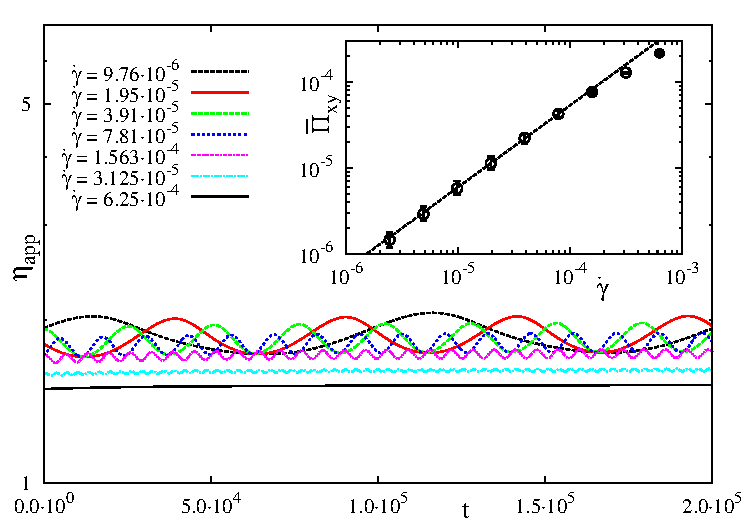
\includegraphics[width=0.495\textwidth]{stress_bp2.pdf}
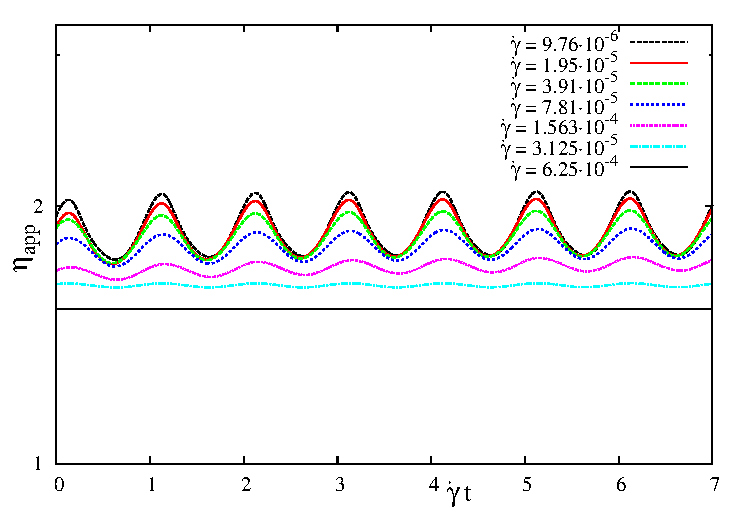
\includegraphics[width=0.495\textwidth]{stress_vs_strain_bp2.pdf}
\caption{Apparent viscosity $\eta_{app}=\Pi_{xy}/\eta\,\gd$ of BPII over time (top) and strain (bottom). For clarity the individual curves have been shifted along the time and strain axis. The inset shows the flow curve $\bar{\Pi}_{xy}(\gd)$ and two different regimes of flow: regular periodic breakup and reconnecting of the discination lines (BPII-1, open circles) and break up of the network into a travelling helical wave (BPII-2, solid circle).}
\label{bp2-rheo}
\end{figure}

We start our discussion with BPII as its flow behaviour turns out to be somewhat simpler 
than that of BPI. BPII has simple cubic symmetry and the $\pi$-disclination lines intersect and form a characteristic network of nodes.

As it might be easier to enter a discussion with the full picture in mind, we provide first a 
quantitative analysis of the flow behaviour at all applied shear rates.
Fig. \ref{bp2-rheo} shows the apparent viscosity, which is defined as the 
deviatoric stress normalised to the isotropic background viscosity: 
$\eta_{app}=\Pi_{xy}/\eta\,\gd$.
A numerical value of $\eta_{app}=1$ corresponds to total shear thinning without 
any additional contribution from the liquid crystal.
The top picutre shows the date over time, whereas the graph at the bottom gives 
the same data versus accummulated strain.
For all but the highest flow rates $\eta_{app}$ oscillates sinusoidally, which
is entirely because of the periodic breakup and reconnecting of the network in shear flow. We refer to this regime as BPII-1.

The inset shows a kind of flow curve, defined as time averages of 
the deviatoric stress tensor $\bar{Pi}_{xy}$ as a function of shear rate $\gd$.
The error bars indicate the maximum and minimum stresses that occur during one cycle.
For all but the largest shear rates a power law fit $\bar{\Pi}_{xy}=a \gd^b$ with 
$a=0.35, b=0.95$ describes the data to a very good approximation. 
Hence, the degree of shear-thinning is remarkably small, but may depend
on the exact direction in which the strain is applied, an aspect that we     
leave for future work.

For shear rates $\gd\ge6.25\e{-4}$ the network of disclination lines
breaks up and oscillations in the stress signal are absent.
In this regime of shear rates, to which we refer as BPII-2, the 
blue phase dissolves into a simple cholesteric liquid 
crystal. The mode of flow is a travelling helical wave with the helical axis 
oriented along the vorticity direction.

In the next paragraph we will investigate this in more detail by looking at the 
kinetics of the disclination network.

\subsubsection{Regime BPII-1: low and intermediate shear rates}

Fig. \ref{bp2-med} shows the disclination network in shear flow as
it undergoes an affine transformation. The disclination lines break up and 
reconnect further downstream forming a periodically recurring pattern with 
recurrence time $\tau_F=1/\gd$ in flow direction.

\begin{figure}[htpb]
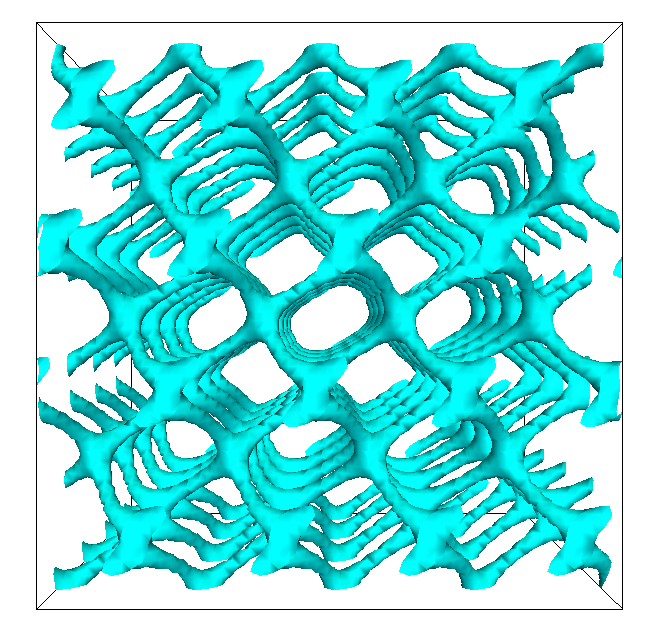
\includegraphics[width=0.4\textwidth]{disc-160k_run902.png}
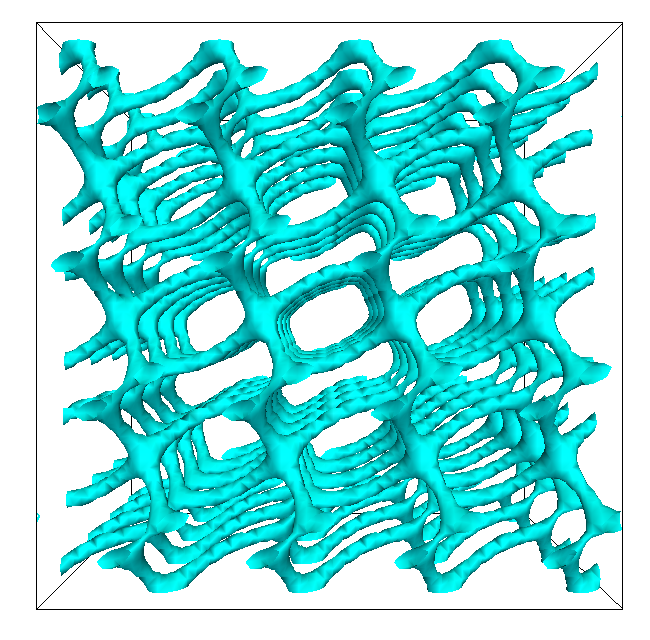
\includegraphics[width=0.4\textwidth]{disc-164k_run902.png}
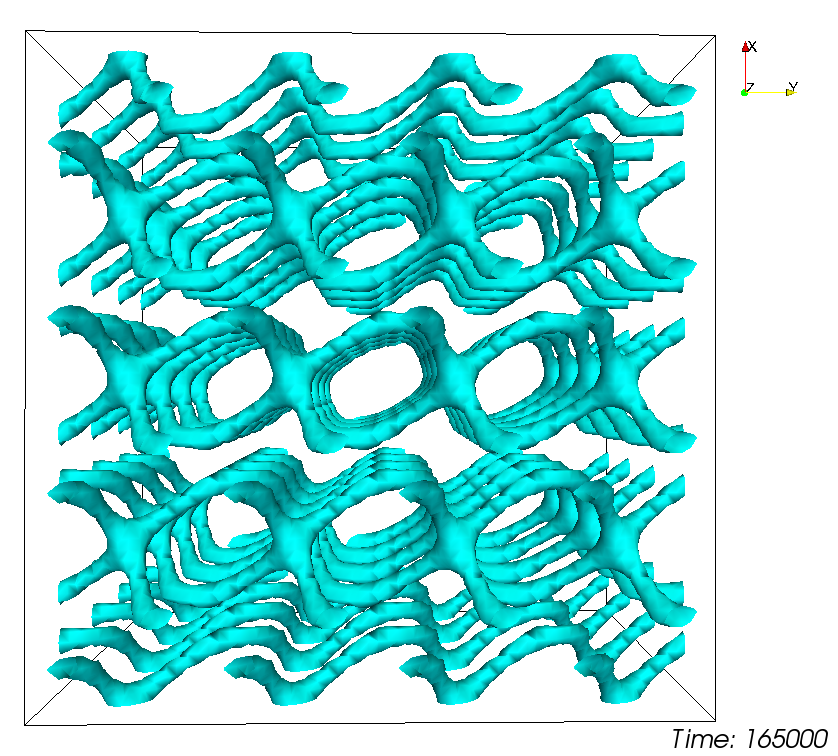
\includegraphics[width=0.4\textwidth]{disc-165k_run902.png}
\caption{Disclination network of BPII in shear flow: 
The pictures show a typical sequence of snapshots in the steady state 
at $\gd=1.56\e{-4}$ and time steps $t=1.60, 1.64,1.65\e{5}$. The velocity 
gradient is oriented along the vertical direction, whereas the 
horizontal direction is the flow direction. Lees-Edwards boundary 
conditions have been imposed in such a way that network moves to the 
right in the upper half and to the left in the lower half of the picture.}
\label{bp2-med}
\end{figure}

\begin{figure*}[htpb]
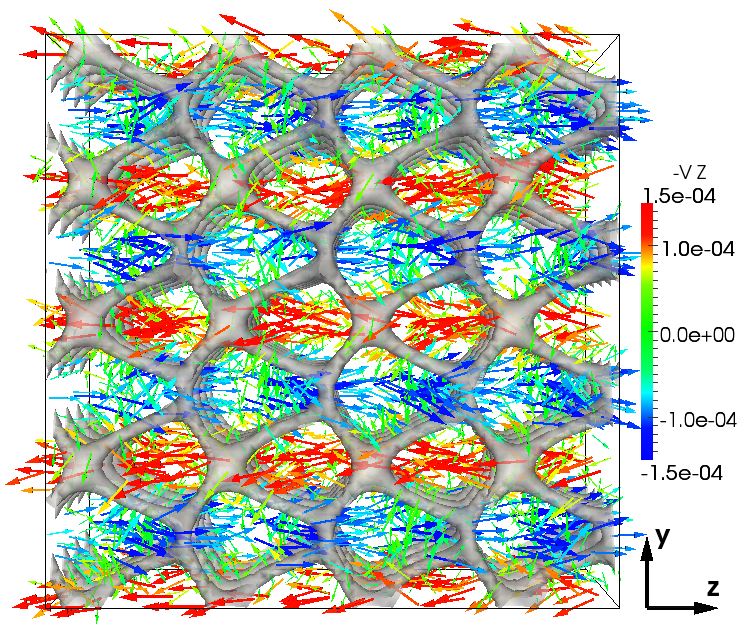
\includegraphics[width=0.495\textwidth]{v_yz-v_z-160k_run902.png}
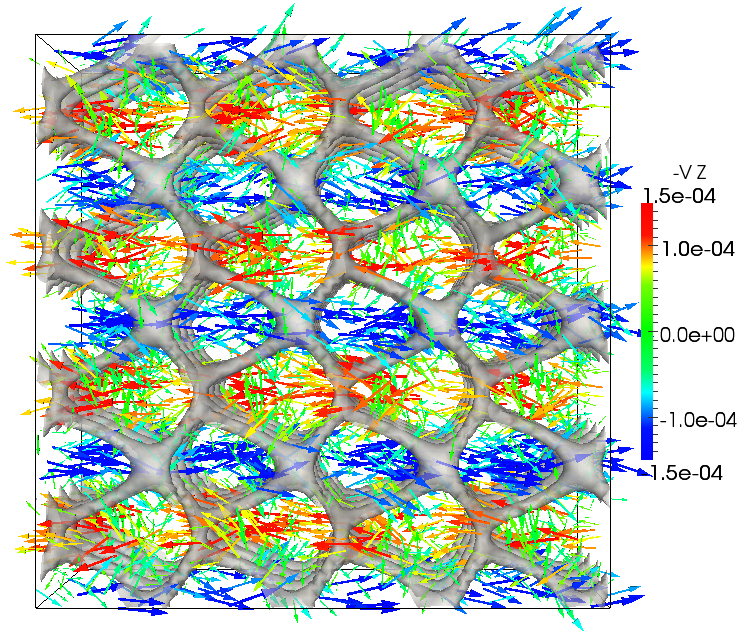
\includegraphics[width=0.495\textwidth]{v_yz-v_z-160k_run903.png}
\caption{Velocity patterns and disclination network in BPII for positive (left) and negative (right) helicity of the 
underlying cholesteric helix: The pictures show velocity vectors $(0,v_y,v_z)$ in x-direction, 
i.e. the velocity has been projected onto a plane perpendicular to the flow direction. 
The vertical and horizontal direction are the gradient and vorticity direction, respectively.
The colour code gives the magnitude and sign of the component in vorticity direction.
The snapshot shows a typical frame during a periodically recurring sequence.
The network on the left with positive helicity travels rightwards, whereas the one one the right
moves leftwards. The recurrence period in vorticity direction is six times longer than the time it takes the network to reconnect in flow direction.}
\label{bp2-velo}
\end{figure*}

The general appearance of the flowing network is apart from the affine transformation 
very close to that of the quiescent blue phase at equilibrium. It is the same for 
all shear rates in regime BPII-1 and a first explanation why shear-thinning is so weak.

Interestingly, while being displaced with the flow the entire network moves perpendicular 
to the flow and velocity gradient in the vorticity direction.
A similar behaviour has been recently observed for blue phases in shear flow and 
confined geometries ~\cite{Henrich:2012b}.
But contrary to the stick-slip motion that has been reported there the movement is 
steady. It occurs in such a manner that the positions of breakup and reconnection 
of the network, visible in Fig. \ref{bp2-med}, are slightly offset and make the network 
travel along the z-direction.
The recurrence time in vorticity direction $\tau_V=6\tau_F$, 
i.e. it takes a displacement of six unit cells in flow directions 
until the network has moved one unit cell in voriticity direction.

Fig. \ref{bp2-velo} shows the disclination network sometime between reconnecting 
and the next breakup with superimposed velocity vectors.
Shown are what we may call secondary velocity components, obtained by projecting the
velocity onto a plain perpendicular to the flow direction.
This allows to get rid of the dominating velocity component $v_x$ and to
visualise the two much smaller components $v_y$ and $v_z$.
The magnitude of the secondary components is typically in the range of a 
few percent of the primary flow component.

Characteristic bands are visible, which are oriented along the vorticity direction and
normally hidden behind the primary flow component.
When the helicity of the underlying cholesteric phase is changed from left- to a 
righthanded the pattern becomes a mirror image of the former one. The sign of 
$v_z$ change and also the sense of motion is inverted.
Further quantitative evidence for a direct link between the sense of motion 
and the helicity can be gained by time-averaging over individual cycles.
Tab. \ref{tab1} gives minima, maxima, averages and standard deviations 
of the velocity components.
All values for the two runs with inverted helicity are identical apart 
from a change of sign in the z-components.
There is only a slight imbalance between the maximum and minimum velocities 
in z-direction, suggesting that the movement of the network in vorticity 
direction is permeative. Note that this imbalance is retained under inversion of
helicity.

\subsubsection{Regime BPII-2: high shear rates}

If the flow rate exceeds a certain critical value BPII does not undergo the 
affine transformation descibed above and adopts another mode of flow. 
Fig. \ref{bp2-high} shows a sequence of cuts through the director 
field at high shear rate. The entire blue phase network has broken up 
into a simple cholesteric helix and flows as a travelling 
helical wave with the helical axis oriented along the vorticity direction.
The state is translationally invariant in flow and gradient direction.
and is the preferred mode of flow of a cholesteric 
liquid crystal at low Ericksen numbers below the uncoiling transition 
to a nematic, flow-aligned state at even higher shear rates ~\cite{Rey:1996a, Rey:1996b}.

In our scenario the break-up occurs for shear rates $\gd>3.12\e{-4}$.
At the moment we do not have a hard criterium for the critical
shear rate at hand. However, it seems reasonable that the critical shear rate 
depends on thermodynamic and kinetic parameters such as the effective 
temperature $\tau$, the chirality $\kappa$ and the rotational diffusion 
constant $\Gamma$.

\begin{figure}[htpb]
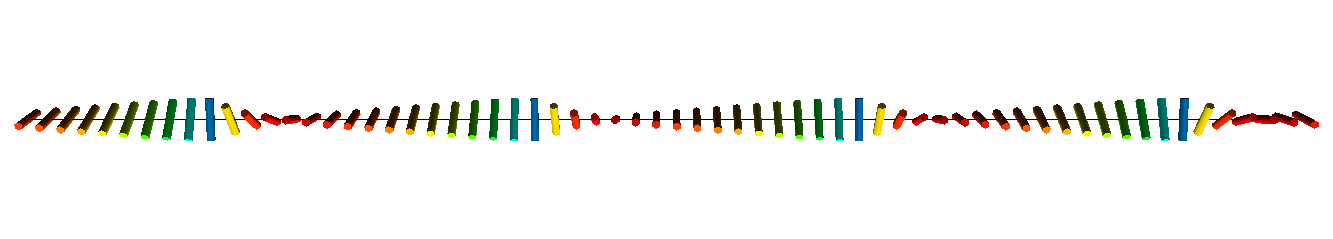
\includegraphics[width=0.495\textwidth]{dir+y-250k_run949.png}
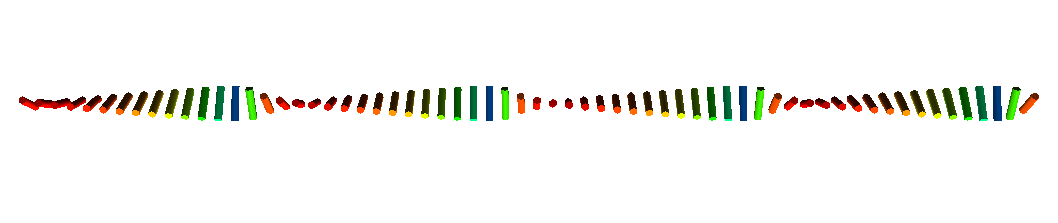
\includegraphics[width=0.495\textwidth]{dir+y-253k_run949.png}
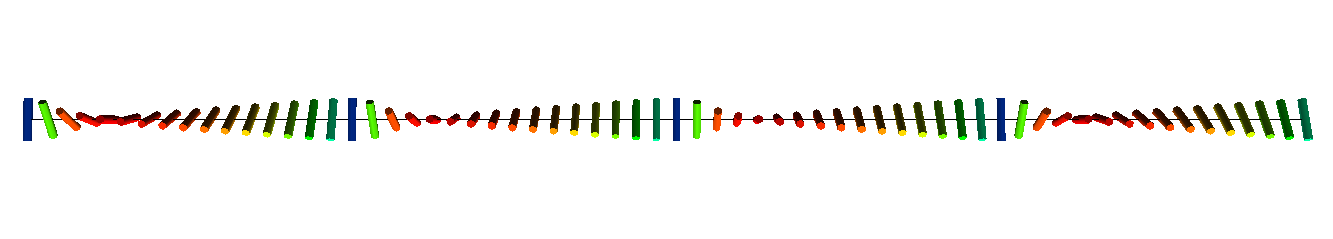
\includegraphics[width=0.495\textwidth]{dir+y-255k_run949.png}
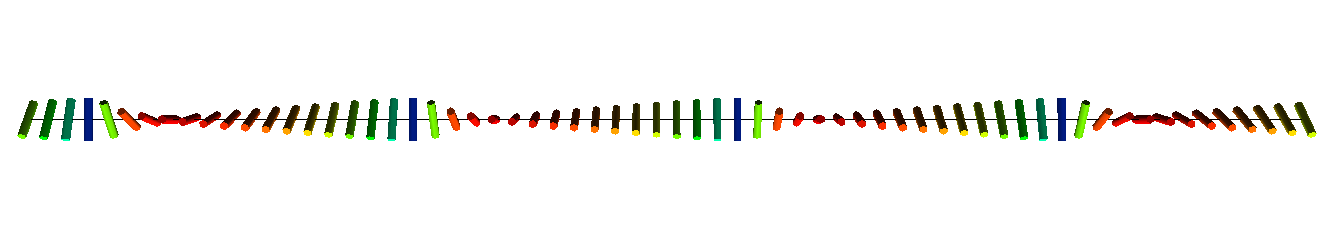
\includegraphics[width=0.495\textwidth]{dir+y-257k_run949.png}
\caption{Director field of BPII at high shear rate: The images show snapshots at time steps 
$t=2.50, 2.53,2.55, 2.57\e{5}$ (from top to bottom) with flow into/out of the page. 
The configuration is a helical wave that travels along the direction of vorticity.
It is translationally invariant in gradient and flow direction.}
\label{bp2-high}
\end{figure}

\subsection{Blue Phase I}

BPI has body-centered symmetry and contrary to BPII the disclination lines
 are well separated and do not intersect.
We believe that this topological difference is responsible for most of
the differences between BPI and BPII regarding their rheological response. 

Again, we present key aspects in a kind of overview before we 
address some features in more detail. Fig. \ref{bp1-rheo} shows the 
apparent viscosity $\eta_{app}$ over time and strain for the same shear rates
as in Fig. \ref{bp2-rheo}.
For shear rates in regime BPI-3, i.e. $\gd\ge6.25\e{-4}$ a breakup of 
the disclination network occurs similar to and at the same critical shear rate as 
the one observed in BPII-2 but with an order structure that is a quasi 
two-dimensional.

In regime BPI-2 at lower shear rates periodic oscillations emerge in the 
deviatoric stress that are not sinusoidal, but show an increasingly complex
pattern up to the breakup point.
For even lower shear rates $\gd\le3.91\e{-5}$ in regime BPI-1 
they become  unregular and finally disappear after a few
cycles. Shear-thinning is slightly stronger than in BPII. 
The average shear stress during one cycle can be fitted reasonably 
well by a power law $\bar{\Pi}_{xy}=a \gd^b$ with $a=0.019, b=0.63$.

\begin{figure}[htpb]
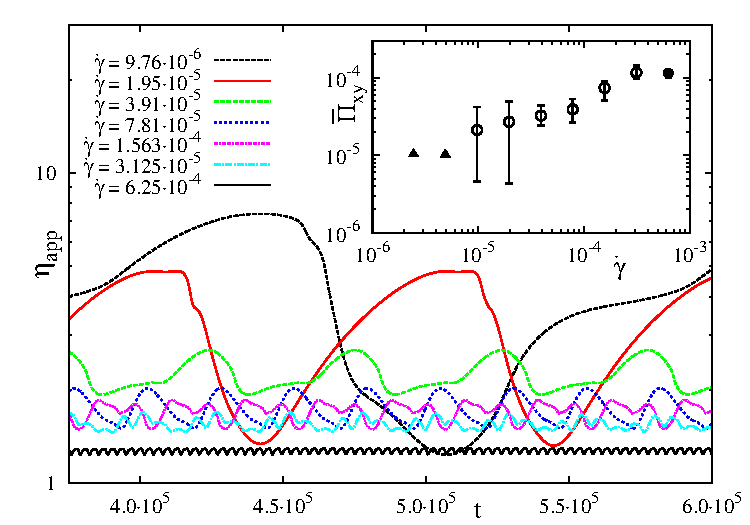
\includegraphics[width=0.495\textwidth]{stress_bp1.pdf}
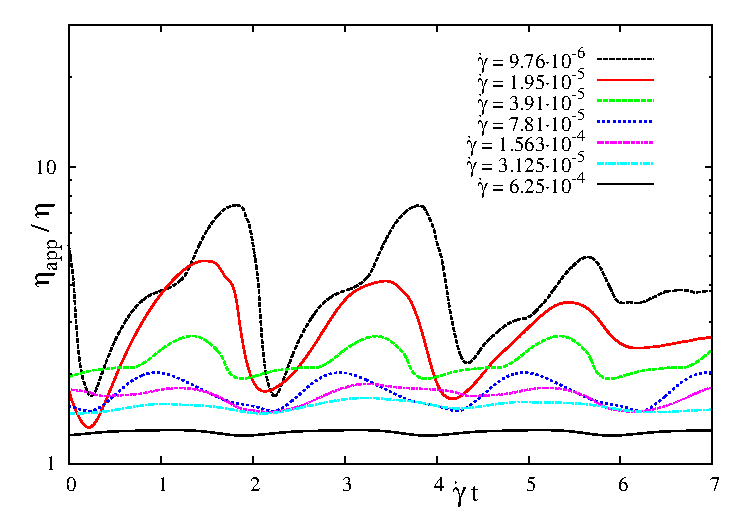
\includegraphics[width=0.495\textwidth]{stress_vs_strain_bp1.pdf}
\caption{Apparent viscosity $\eta_{app}=\Pi_{xy}/\dot{\gamma}$ of BPI over time (top) 
and strain (bottom). The inset shows the flow curve $\bar{\Pi}_{xy}(\gd)$. 
Depending on the configuration in steady shear flow three different regimes 
can be identified: amorphous BP network with yield stress (BPI-1, triangles), 
steady flow with recurring patterns (BPI-2, open circles) and 
breakup of the disclination network (BPI-3, solid circle). 
The error bars represent the minimum and maximum shear stress 
during one cycle. For clarity the individual curves have been shifted along
the time and strain axis.}
\label{bp1-rheo}
\end{figure}

The Fourier analysis of the time-dependent deviatoric stress $\Pi_{xy}$ 
offers another perspective on this intricate flow behaviour at high and intermediate shear rates. 
The spectrum $X_\omega$ according to Eq. \ref{spectrum} is shown in Fig. \ref{bp1-spectrum}.
We observe a strong contribution of the first harmonic, which is directly related to the 
recurrence period $T$, shear rate $\dot{\gamma}$ and unit cell size $l_{u}$ 
via $\omega_0=2\pi/T=2\pi/(l_{u}\dot{\gamma})$.
As the shear rates we applied always differ by a factor 2 the Fourier coefficients of the 
individual runs with different shear rate coincide in such a way that the
the fundamental mode is the same frequency as the first overtone of the next lower shear rate
or the third overtone of the next-to-next lower shear rate 
(viz. peak positions at $\gd=7.81, 3.91$ and $1.95\e{-5}$).
Moreover, the magnitude of higher Fourier modes decreases monotonously.   
However, the inset shows that this characteristic frequency relation is violated 
for shear rates above $\gd=7.81\e{-5}$.
Although the velocity of the primary flow component in x-direcition, listed in Tab. \ref{tab1},
 is very well in accordance with the imposed shear rate, the fundamental mode appears 
now at the same frequency.
The contribution of higher Fourier modes increases and even exceeds that of
the fundamental mode, which gives the shear stress generally a more jittering appearance.
At the highest imposed shear rate where the breakup occurs the Fourier spectrum 
becomes simple again and features a dominating fundamental mode at the 
expected frequency just as described above for $\gd\le7.81\e{-5}$.
The breakup occurs at exactly the same flow rate as those of BPII, 
suggesting that this can be traced back to the rotational dynamics 
of the order parameter.

\begin{figure}[htpb]
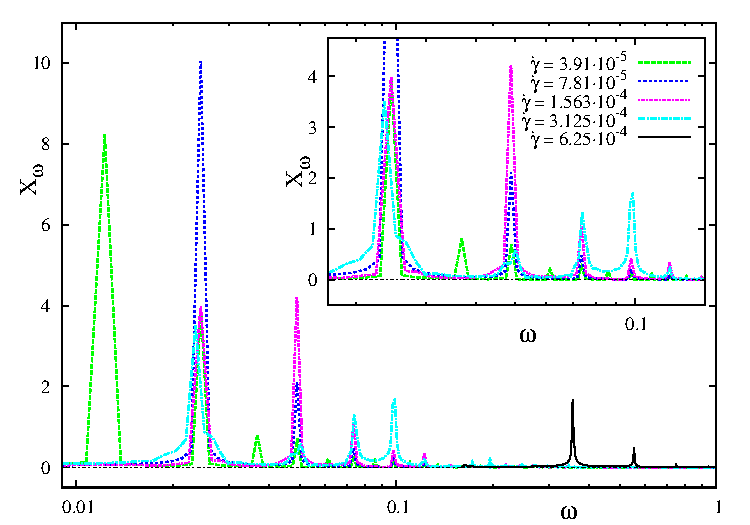
\includegraphics[width=0.495\textwidth]{spectrum_bp1.pdf}
\caption{Fourier analysis of the deviatoric stress $\Pi_{xy}$ of BPI at different shear rates: The main picture shows the frequency shift of the Fourier components in agreement with the imposed shear rate. The inset depicts the same analysis at higher shear rate, where the frequency shift is no longer observed. Instead the spectral contribution of higher modes grows until finally the breakup takes place. The frequency is given in units of $10^2\cdot 2\pi/T$ with $T$ as period of one cycle in LB time steps.}
\label{bp1-spectrum}
\end{figure}

\subsubsection{Regime BPI-1: low shear rates}

The rheological response of BPI at low shear rate which exhibits a
dynamic yield stress is strikingly different from that of BPII.
An explanation for this strange behaviour can be found by 
looking more closely at the average deviatoric stress and 
free energy density, as shown in Fig. \ref{bp1-fe-yield}.
When the quiescent and equilibrated BPI network begins to flow
the shear stress increases steeply and goes through a global maximum.
Shortly after it goes negative (the total shear stress is still
positive as the backgound viscosity has been subracted) and positive
again, forming a complete cycle. 
This cycle is repeated for a couple of times before 
the amorphous configuration emerges and any regular pattern
disappears.
The negative branch in the deviatoric stress is connected
to a local maximum followed by a local minimum in the average free energy.
Hence, the region of negative stress can be 
regarded as a phase during which elastic forces excert a 
'pull' onto the network while it tries to reach a more 
favourable configuration. However, the low flow rate
causes this unstable intermediate state to be exposed to these
pulling elastic forces for a relatively long time, long enough to 
create small distortions which finally break the symmetry of the
flow-induced configuration.

\begin{figure}[htpb]
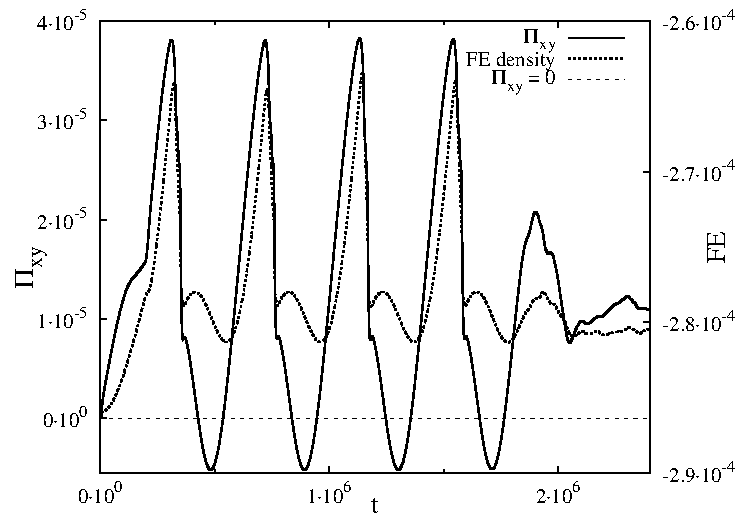
\includegraphics[width=0.495\textwidth]{stress_fe_yield_bp1.pdf}
\caption{Average deviatoric stress and free energy density of BPI at low shear rate: The negative branch in the stress is related to a local maximum and a following local minimum in free energy density. This creates unstable conditions that lead to a dissolving regular network and an amorphous state which features a yield stress.}
\label{bp1-fe-yield}
\end{figure}

We want to explain these differences on the basis of a typical 
appearance of BPI at low flow rate, which is depicted in Fig. \ref{bp1-low}.
Three different stages can be distinguished. 
With the onset of shearing the disclination lines 
in BPI get more and more squeezed together which is incommensurable with 
the defect topology of this blue phase. 
Consequently, the network adopts a flow-induced conformation which consists 
of intertwined helices that stretch during the affine transformation.
This helical conformation that emerges already at strains $\gamma\simeq1$ 
is shown in Fig. \ref{bp1-low} (top row).
At a particular point in the cycle a non-helical configuration is
observed (bottom left) before the network quickly returns
to its helical state.
There is no perceivable movement of the network in vorticity 
direction at any stage of the cycle.


\begin{figure*}[htpb]
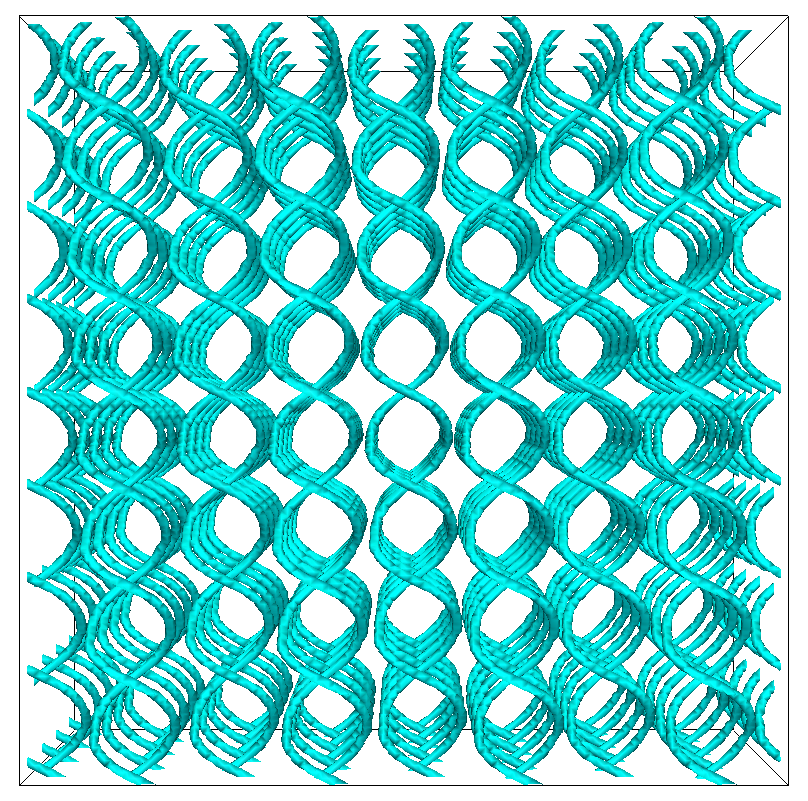
\includegraphics[width=0.32\textwidth]{disc-xy-400k_run1115.png}
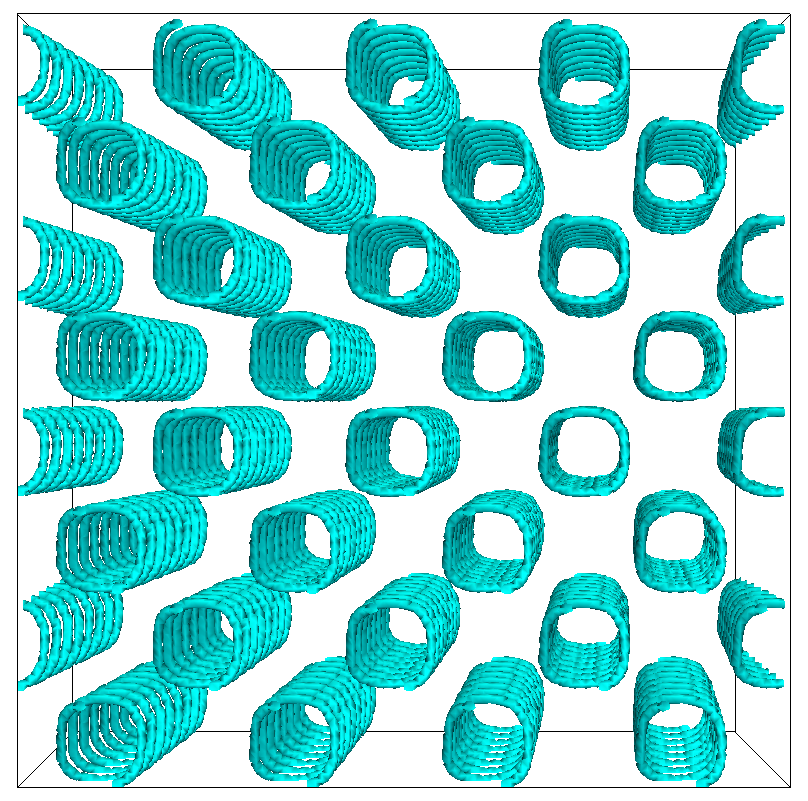
\includegraphics[width=0.32\textwidth]{disc-yz-400k_run1115.png}
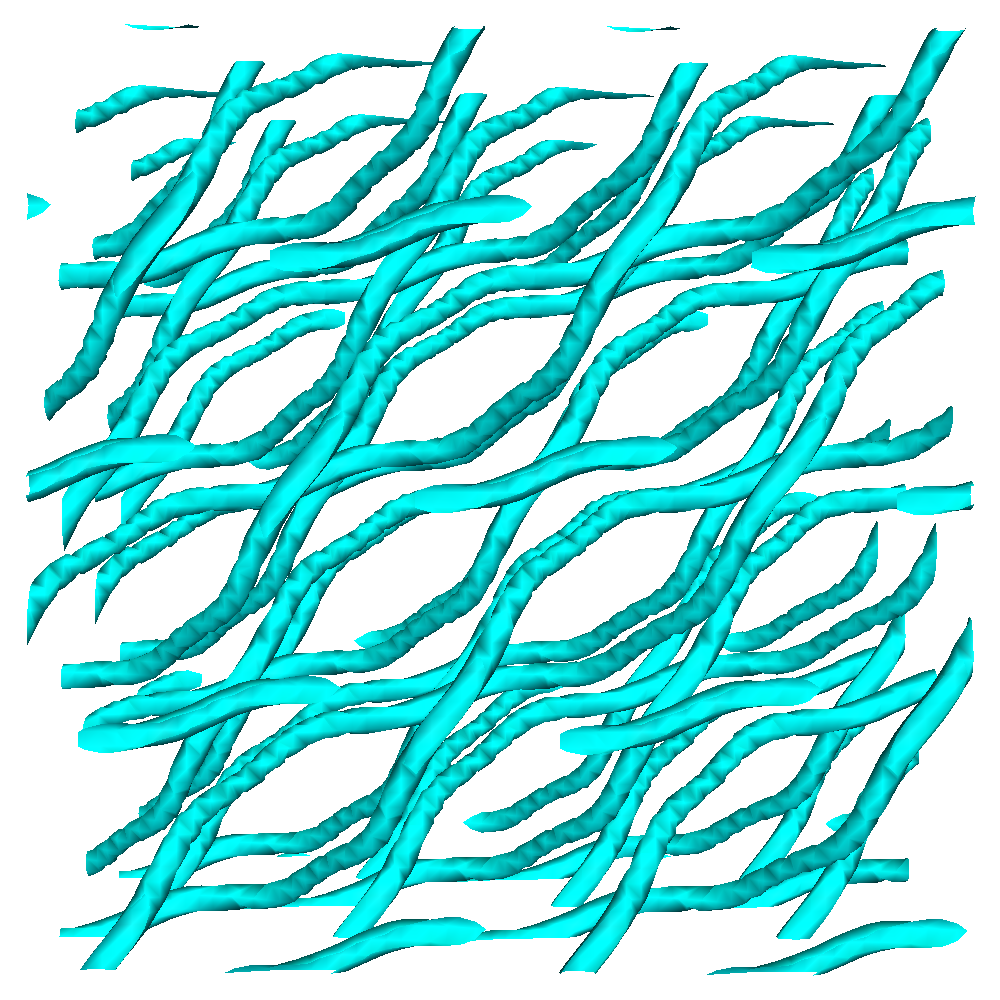
\includegraphics[width=0.32\textwidth]{disc-xy-700k_run1115.png}\\
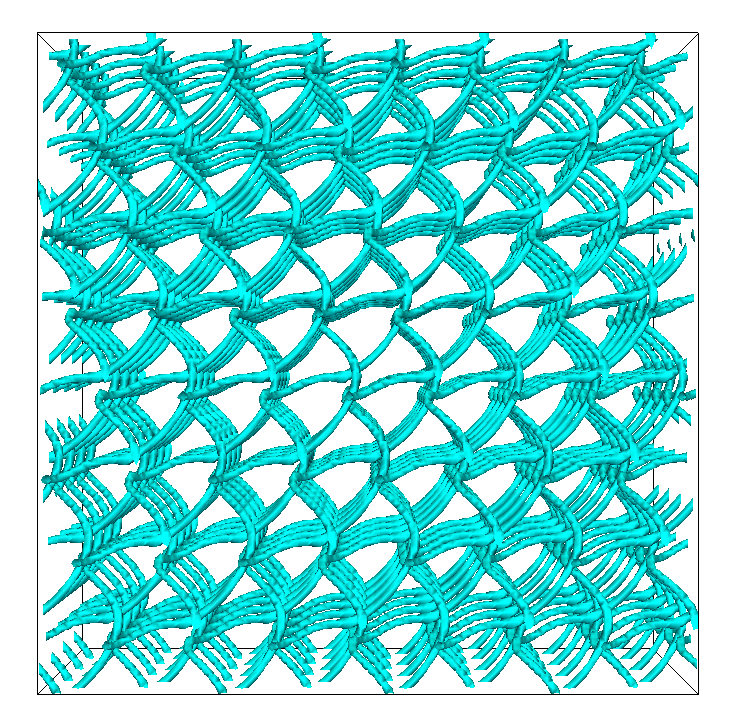
\includegraphics[width=0.32\textwidth]{disc-xy-750k_run1115.png}
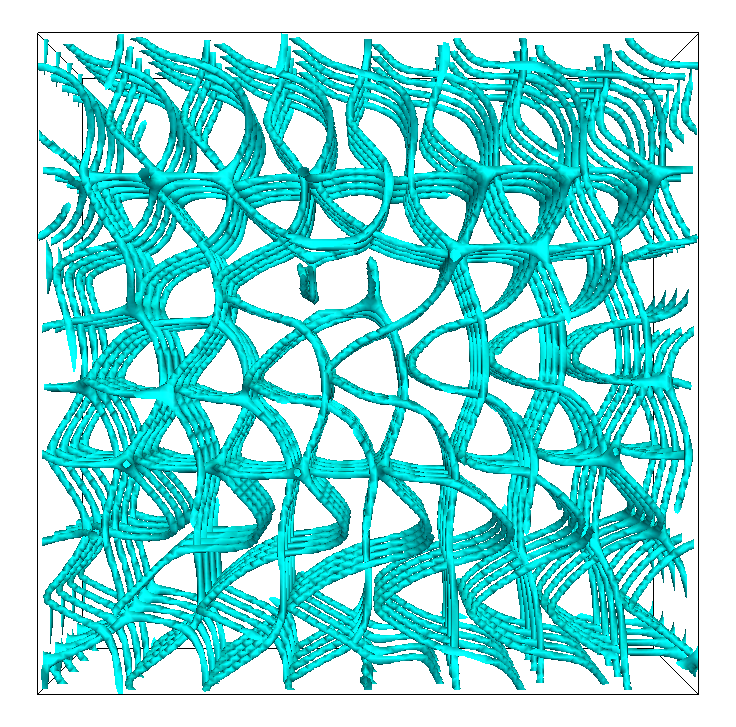
\includegraphics[width=0.32\textwidth]{disc-xy-1700k_run1115.png}
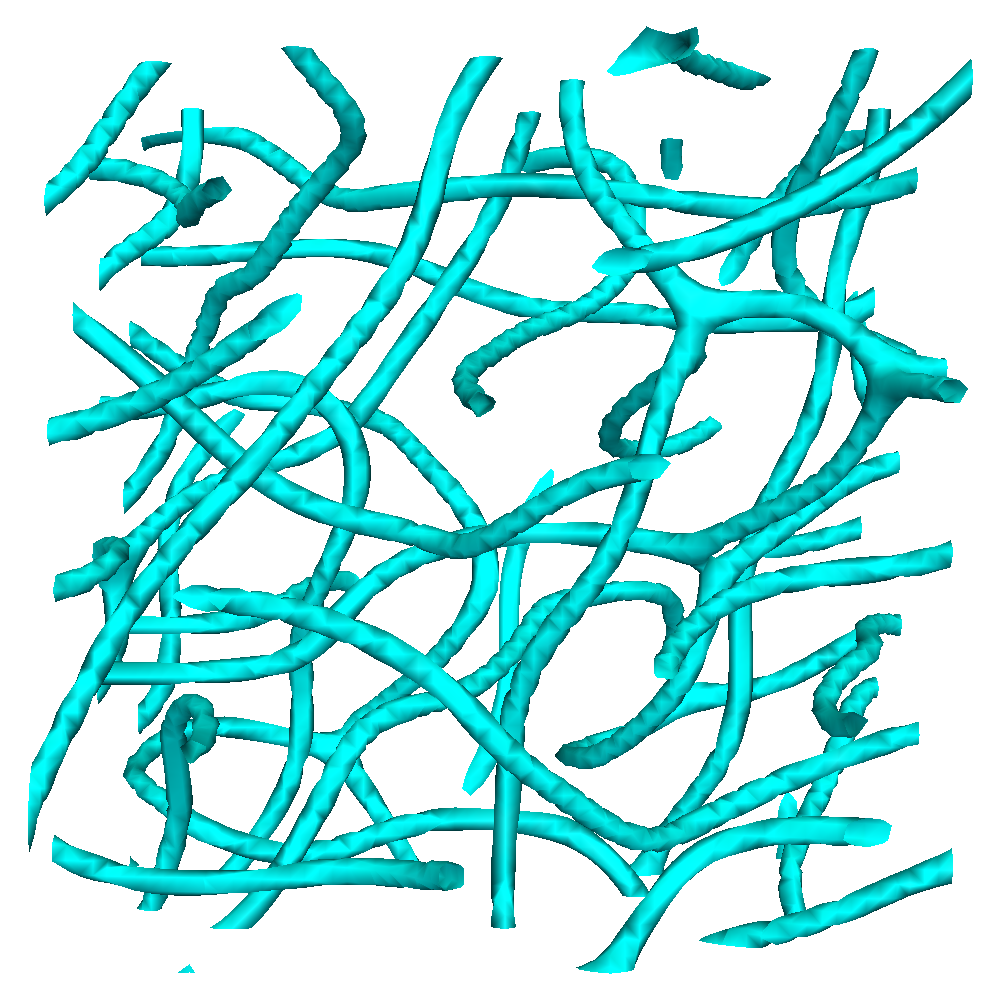
\includegraphics[width=0.32\textwidth]{disc-xy-2200k_run1115.png}
\caption{Snapshots of BPI disclination network at low shear rate ($\dot{\gamma}=4.88\e{-6}$): Depicted is the transition from flow-induced, intertwined helices that undergo a recurring affine transformation (top left and centre at time step $t=4.0\e{5}$, top right at $t=7.0\e{5}$) with an intermediate conformation that is non-helical (bottom left at time step $t=7.5\e{5}$) to a distorted state (bottom centre at time step $t=1.7\e{6}$) and finally to an amorphous network (bottom right at $t=2.2\e{6}$). All pictures have the vie along the vorticity direction apart from the one at the top centre which shows the network in gradient direction.}
\label{bp1-low}
\end{figure*}

However, this mode of flow proves unstable as after a few cycles 
distortions appear which lead to further destabilisation.
Finally, the network loses any residual order and 
transforms into an amorphous state with virtually constant
yield stress in the region of $\Pi_{xy}\simeq 1\e{-5}$ in LU.

\subsubsection{Regime BPI-2: intermediate shear rates}

Intermediate shear rates in the sense of this study of BPI are characterised 
by the missing negative branch in the deviatoric stress. It is unclear 
why this feature is missing at higher flow rates. A possible explanation is that 
above a certain flow rate the network simply skips the comparably small 
window of negative stress in Fig. \ref{bp1-fe-yield} and finds a quicker 
route to get back on the positive branch.

\begin{figure}[htpb]
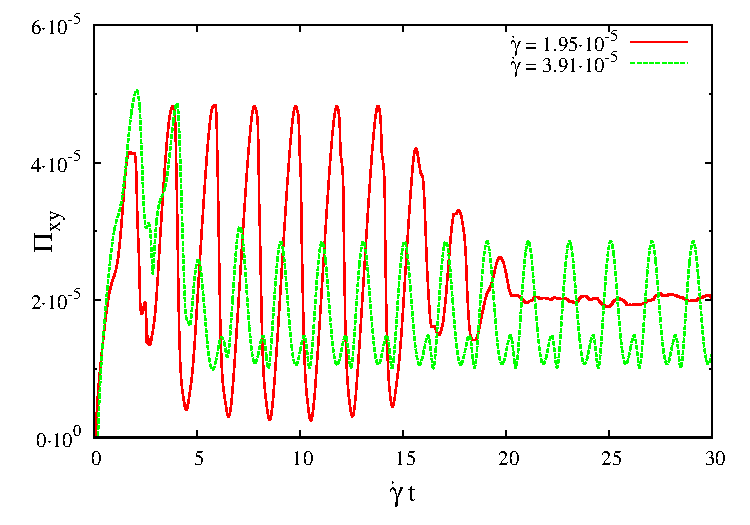
\includegraphics[width=0.495\textwidth]{stress_bp1-1_bp1-2.pdf}
\caption{}
\label{bp1-1_bp1-2}
\end{figure}

Fig. \ref{bp1-med} shows snapshots of BPI in steady shear flow. 
Contrary to BPII the flow-induced conformations of BPI differ significanly 
from the appearance of BPI at equilibrium. The depicted 
state is rather surprisingly still kinematically connected to the equilibrium state.
When the shear flow is switched off the flow-induced configuration reverts
to its original configuration of a BPI network at rest.
%%%%%%%%%%%%
%The recurrence time in flow direction is $\tau_F=L_x/(2\, v_{LE})=L_x/(2\,\gd\, \Delta y_{LE})= 4/\gd$.
%%%%%%%%%%%
After each cycle the position of the network is displaced with respect to the beginning of the cycle.
However, neither the magnitude nor the direction of the offset obey a clear rule,
are different and non-integer for every shear rate in this regime of flow. 
This suggests the described phenomenon constitutes an instance of rheochaos in this 
regime of liquid crystalline flow. 

\begin{figure*}[htpb]
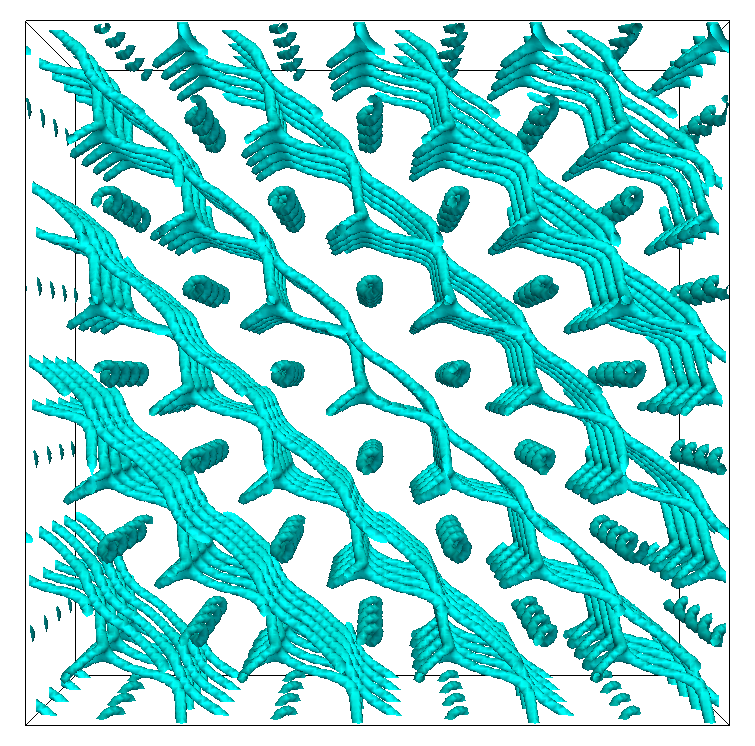
\includegraphics[width=0.32\textwidth]{disc-365k_run914.png}
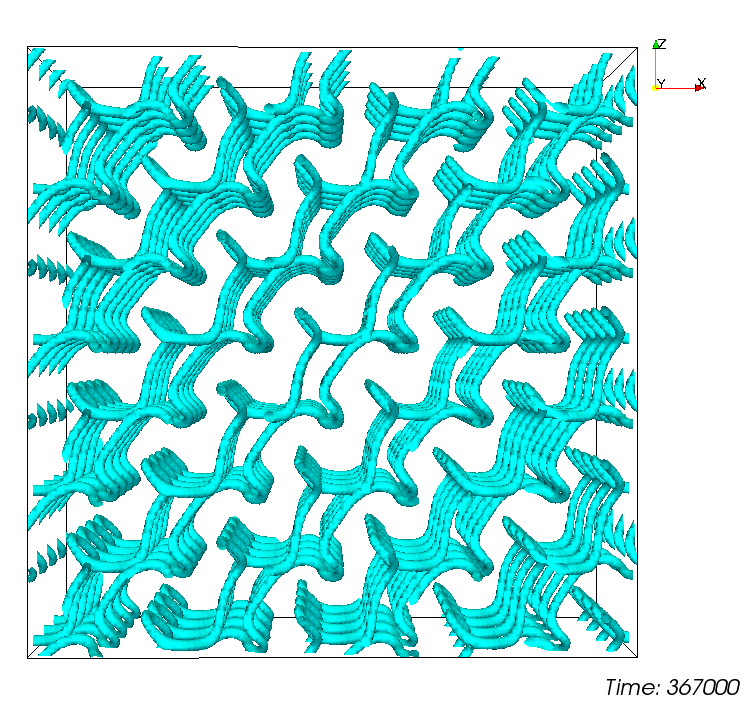
\includegraphics[width=0.32\textwidth]{disc-367k_run914.png}
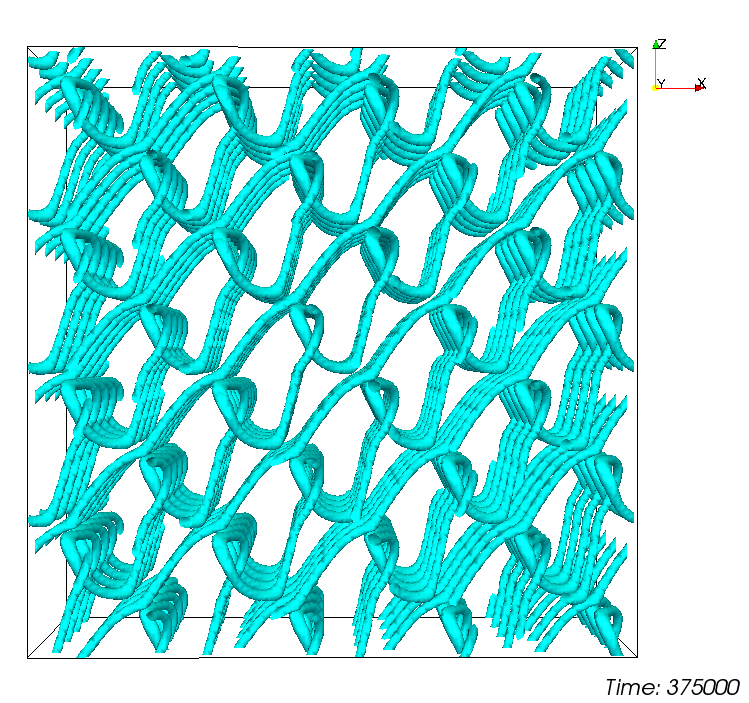
\includegraphics[width=0.32\textwidth]{disc-375k_run914.png}\\
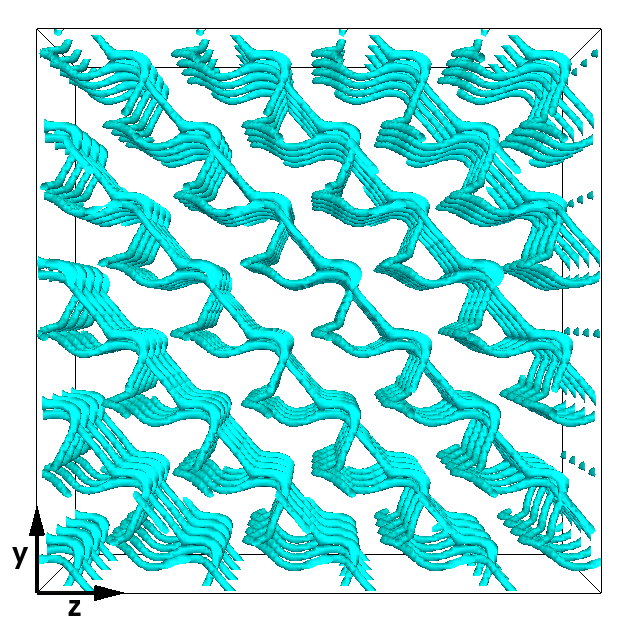
\includegraphics[width=0.32\textwidth]{disc-380k_run914.png}
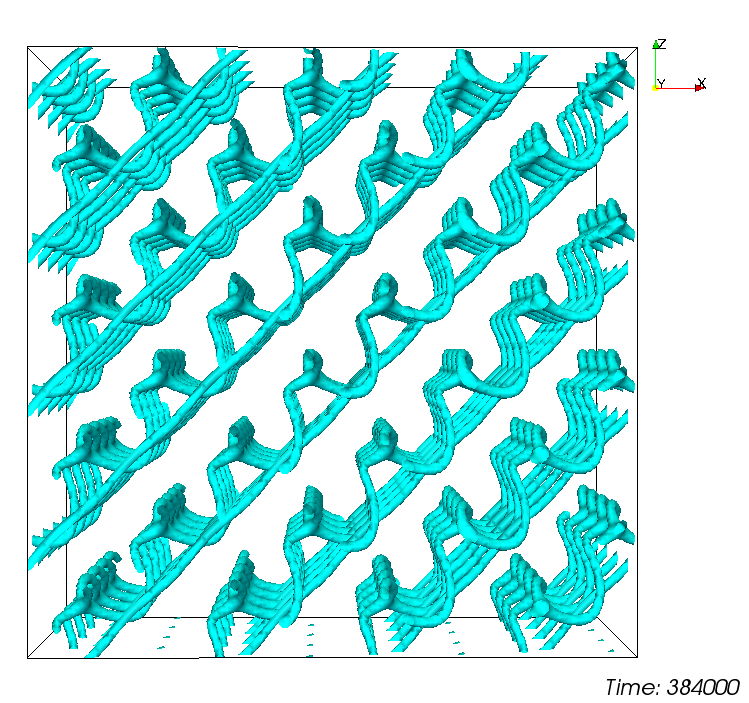
\includegraphics[width=0.32\textwidth]{disc-384k_run914.png}
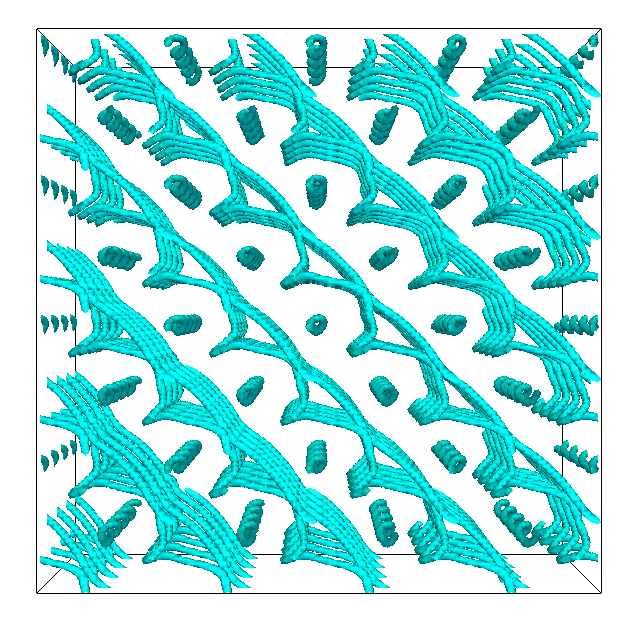
\includegraphics[width=0.32\textwidth]{disc-389k_run914.png}
\caption{Disclination network of BPI at intermediate flow rates: The pictures show a typical sequence of shear-induced transformations in the steady state at $\gd=1.56\e{-4}$ and time steps $t=3.65, 3.67,3.75,3.80,3.84,3.89\e{5}$ with the flow into/out of the page. The network is displaced during every cycle, but the magnitude and direction of the offset appear to be chaotic.}
\label{bp1-med}
\end{figure*}

Fig. \ref{bp1-velo} depicts the secondary velocity components $v_y$ and $v_z$ in the same fashion as Fig. \ref{bp2-velo} for BPII. Again, the orientation of the components are as mirror images of each other if the helicity of the cholesteric changes from left- to right-handed.
The emerging pattern is different from the one observed before in BPII, but agrees with
the previous result in the sense that secondary velocities are largest in the regions
where large conformational changes take place. 

\begin{figure*}[htpb]
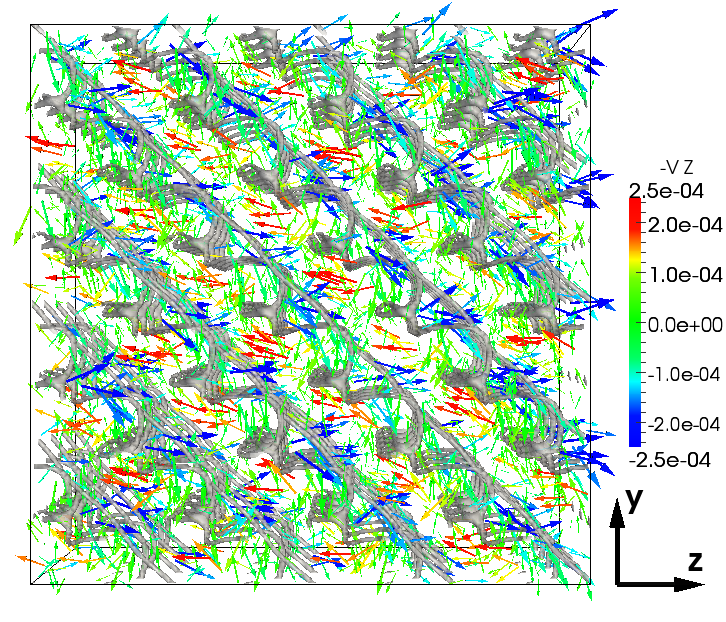
\includegraphics[width=0.495\textwidth]{v_yz-v_z-360k_run914.png}
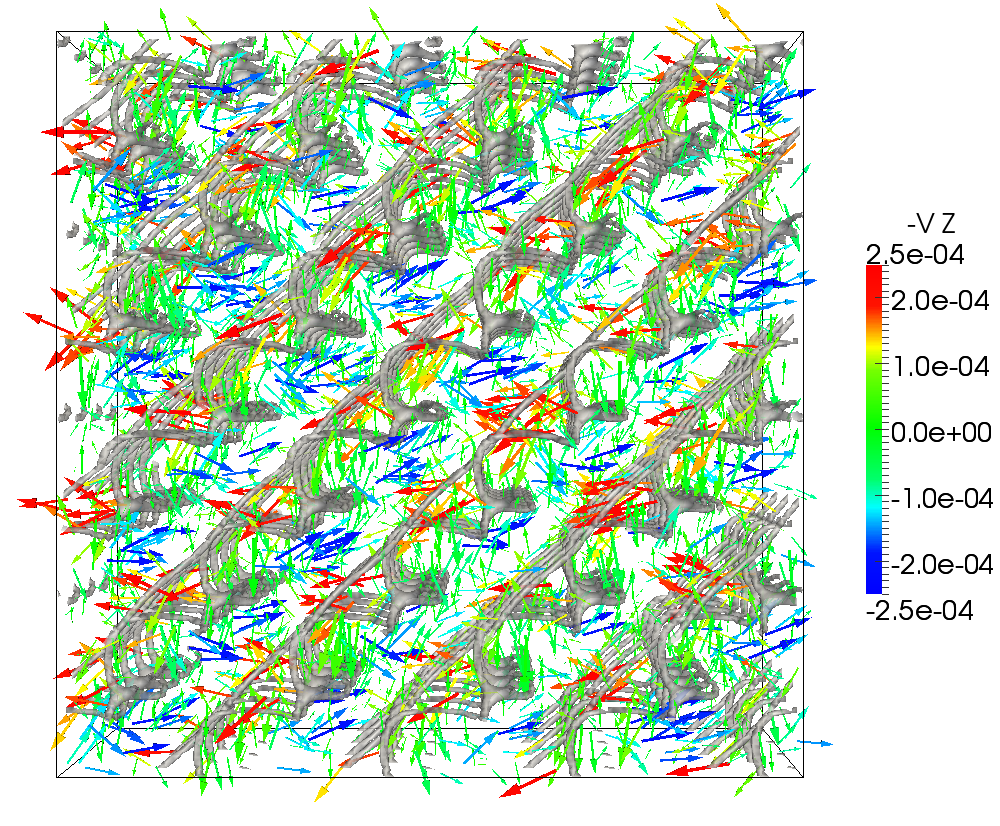
\includegraphics[width=0.495\textwidth]{v_yz-v_z-360k_run922.png}
\caption{Velocity patterns in BPI for positive (left) and negative (right) helicity: The pictures show a snapshot of the periodically recurring sequence and velocity vectors $(0,v_y,v_z)$ with the component in flow direction set to zero. The colour code gives the magnitude and sign of the z-component. The vertical and horizontal direction are the gradient and vorticity direction, respectivelty. Flow occurs in such a way that the network moves into (out of) the paper plane in the upper (lower) half of the images.}
\label{bp1-velo}
\end{figure*}

The complexity of flow-induced states and the seemingly chaotic but 
periodic movement of the BPI network raises the question how robust 
these results are with respect to the system size.
Although the pitch length of 64 LU and the equivalent of 32 LU per
unit cell provide enough resolution to track the motion of the 
network in flow it is not clear whether 64 unit cells in total are enough to 
mimick true bulk behaviour. 

Unfortunately the computational costs are still prohibitive for a run 
with 512 unit cells, an equivalent of 8 unit cells along each coordinate 
direction. Therefore we opted for a comparison with a smaller run consiting
of 8 unit cells, 2 along each dimension.
Fig. \ref{bp1-2uc4uc} shows a comparison of the apparent viscosity $\eta_{app}$ 
of runs with 8 and 64 unit cells at flow rates 
$\gd=9.76\e{-6}$ and $1.95\e{-5}$, respectively.
We do not visualise the conformations directly but rather use the fact that 
they are coded in the shape of each individual curve. Obviously there 
are stiking differences between 
both system sizes, but the recurrence period is hardly affected. In the slower
run the smaller system apparently follows the same branch for a while but then
deviates from the larger run. 
This result indicates that we cannot know with certainty if the particular flow patterns 
we find at runs with 64 unit cells do not suffer from the imposed periodicity.
Nevertheless, the chaotic behaviour and the recurrency seem to be a generic
feature of BPI in this flow regime.
 
\begin{figure}[htpb]
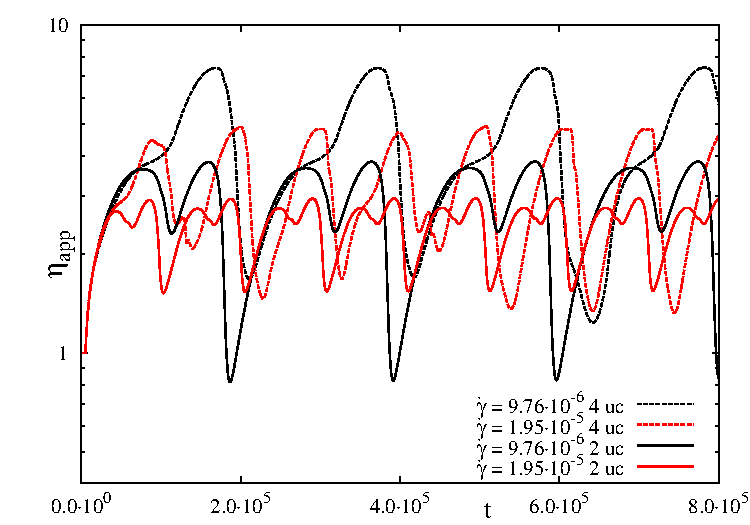
\includegraphics[width=0.495\textwidth]{stress_bp1_2uc_4uc.pdf}
\caption{Apparent viscosity $\eta_{app}$ for 8 (solid lines) and 64 unit cells (dashed lines)
at $\gd=9.76\e{-6}$ and $1.95\e{-5}$. The shape of each curve differs largely, but the recurrence frequencies are hardly affected by the system size.}
\label{bp1-2uc4uc}
\end{figure}

\subsubsection{Regime BPI-3: high shear rates}

\begin{figure}[htpb]
%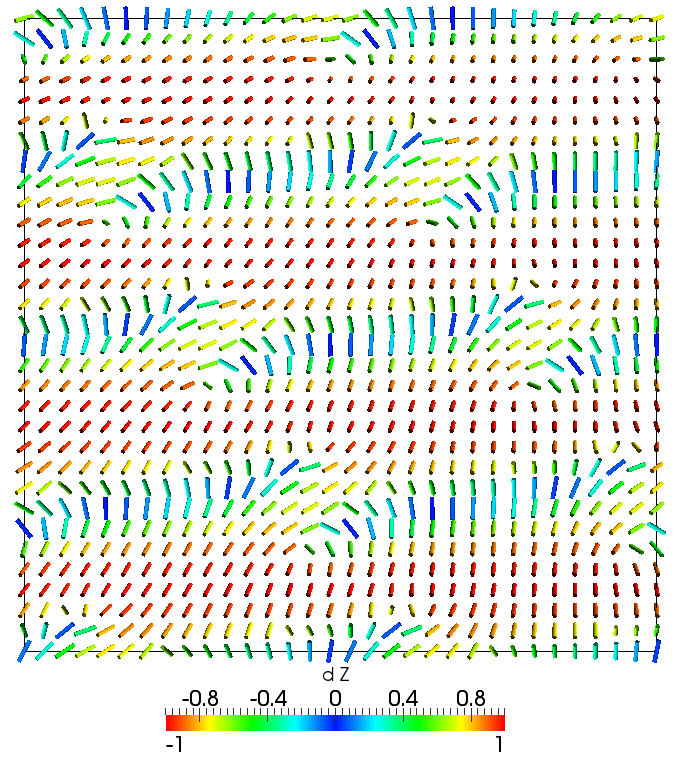
\includegraphics[width=0.4\textwidth]{dir+z-300k_run916.png}
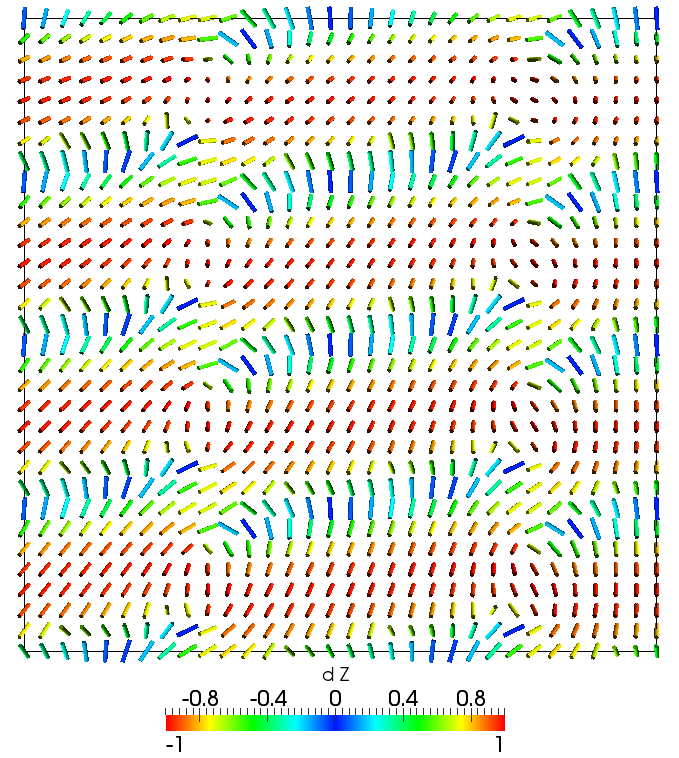
\includegraphics[width=0.4\textwidth]{dir+z-301k_run916.png}
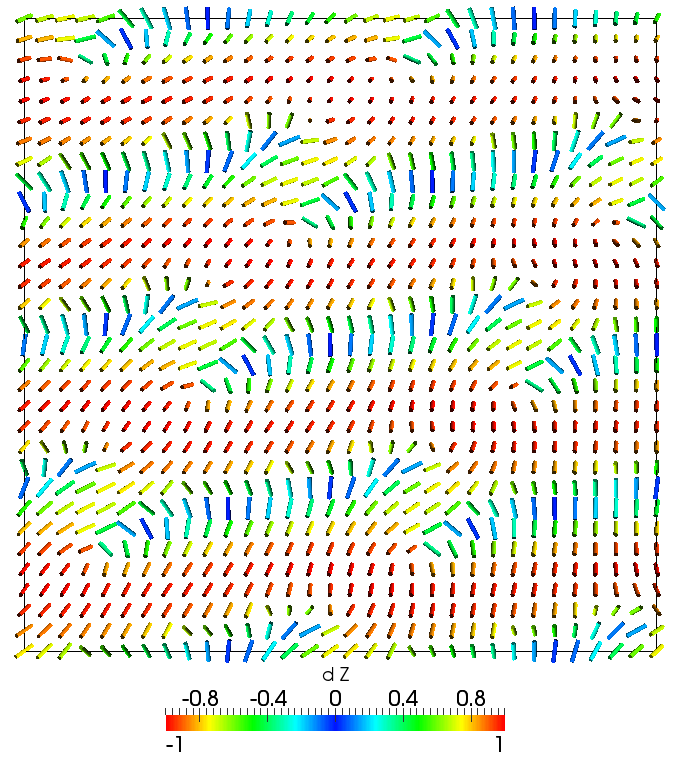
\includegraphics[width=0.4\textwidth]{dir+z-302k_run916.png}
\caption{Director field of BPI at high shear rate: The pictures show a slice of $L_x\times L_y = 64\times64$ lattice sites along the vorticity direction with the flow / gradient direction oriented along the horizontal / vertical axis. The colour code gives the magnitude of the in-plane component of the director field. The data is translationally invariant in vorticity direction.}
\label{bp1-high}
\end{figure}
 
A breakup of the network at large flow rates is also observed
in BPI. Interestingly the window of critical shear rates 
$3.125\e{-4}\le\gd_c\le 6.25\e{-4}$  is the same we find for BPII.  
Contrary to BPII, which flows in form of a travelling helical wave
(viz. Fig. \ref{bp2-high}) the preferred configuration is now
a quasi two-dimensional state, shown in Fig. \ref{bp1-high} as 
slices through the director field along the voritcity direction.      
The sequence shows that BPI undergoes the affine transformation 
in gradient-flow plane often seen in simple shear flow.
There are distinctive regions where the predominant orientation 
of the director is along the vorticity direction and others
where it lies in flow-gradient plane. Occasionally while 
flowing past each other this produces regions that 
resemble local double twist.




\clearpage

\section{Conclusions}

% If in two-column mode, this environment will change to single-column
% format so that long equations can be displayed. Use
% sparingly.
%\begin{widetext}
% put long equation here
%\end{widetext}

% figures should be put into the text as floats.
% Use the graphics or graphicx packages (distributed with LaTeX2e)
% and the \includegraphics macro defined in those packages.
% See the LaTeX Graphics Companion by Michel Goosens, Sebastian Rahtz,
% and Frank Mittelbach for instance.
%
% Here is an example of the general form of a figure:
% Fill in the caption in the braces of the \caption{} command. Put the label
% that you will use with \ref{} command in the braces of the \label{} command.
% Use the figure* environment if the figure should span across the
% entire page. There is no need to do explicit centering.

% \begin{figure}
% \includegraphics{}%
% \caption{\label{}}
% \end{figure}

% Surround figure environment with turnpage environment for landscape
% figure
% \begin{turnpage}
% \begin{figure}
% \includegraphics{}%
% \caption{\label{}}
% \end{figure}
% \end{turnpage}

% tables should appear as floats within the text
%
% Here is an example of the general form of a table:
% Fill in the caption in the braces of the \caption{} command. Put the label
% that you will use with \ref{} command in the braces of the \label{} command.
% Insert the column specifiers (l, r, c, d, etc.) in the empty braces of the
% \begin{tabular}{} command.
% The ruledtabular enviroment adds doubled rules to table and sets a
% reasonable default table settings.
% Use the table* environment to get a full-width table in two-column
% Add \usepackage{longtable} and the longtable (or longtable*}
% environment for nicely formatted long tables. Or use the the [H]
% placement option to break a long table (with less control than 
% in longtable).
% \begin{table}%[H] add [H] placement to break table across pages
% \caption{\label{}}
% \begin{ruledtabular}
% \begin{tabular}{}
% Lines of table here ending with \\
% \end{tabular}
% \end{ruledtabular}
% \end{table}

% Surround table environment with turnpage environment for landscape
% table
% \begin{turnpage}
% \begin{table}
% \caption{\label{}}
% \begin{ruledtabular}
% \begin{tabular}{}
% \end{tabular}
% \end{ruledtabular}
% \end{table}
% \end{turnpage}

% Specify following sections are appendices. Use \appendix* if there
% only one appendix.
%\appendix

%\section{}

% If you have acknowledgments, this puts in the proper section head.
\begin{acknowledgments}
Thanks folks!
\end{acknowledgments}

% Create the reference section using BibTeX:
\bibliography{bprheo}

\end{document}
%
% ****** End of file apstemplate.tex ******

